\subsection{Translational Controller}
The translational controllers are structured as cascade loops, where the velocity and position are controlled in the inner and outer loop, respectively. The relation between the controllers is presented in \autoref{fig:cascade}.
%
\begin{figure}[H]
	\hspace{-.37cm}
	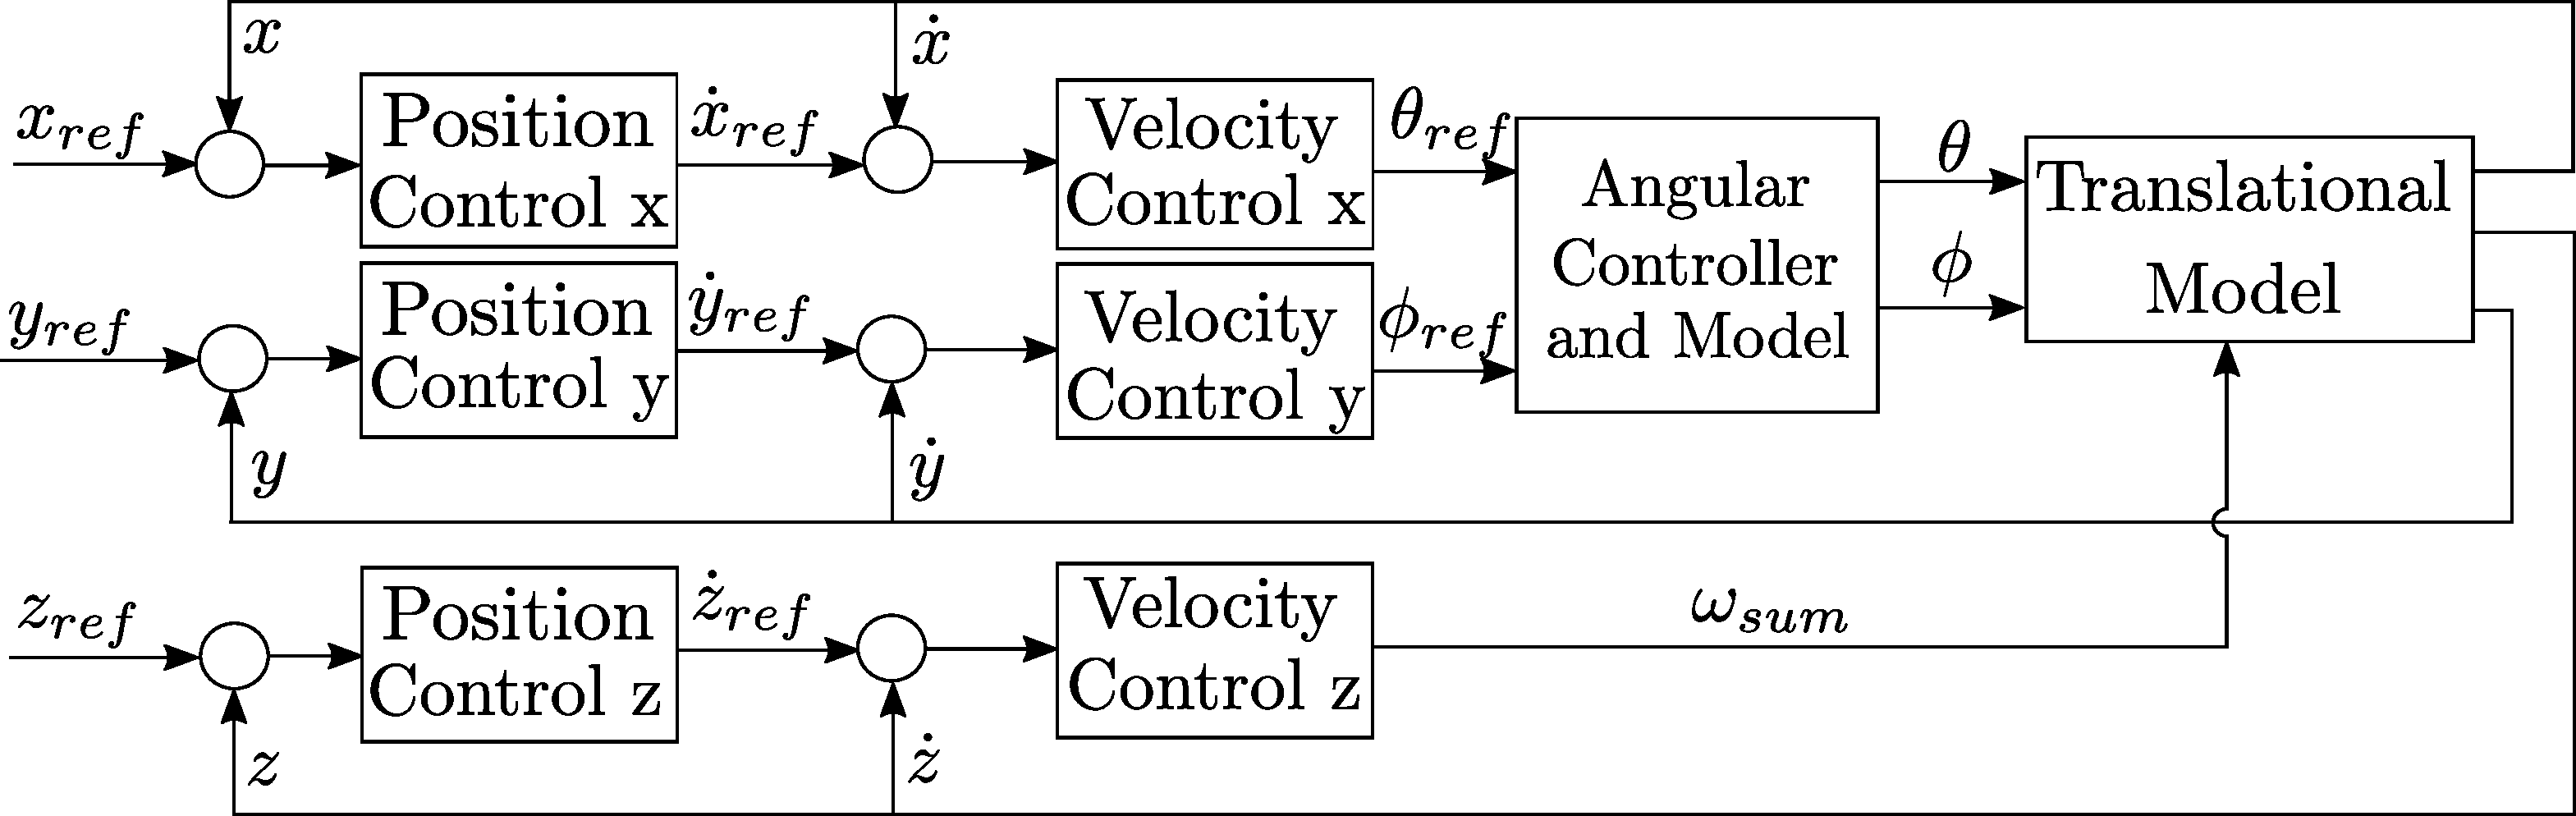
\includegraphics[width=.54\textwidth]{figures/TranslationalControlDiagram.pdf}
	\caption{Overview of translational controllers structure.}
	\label{fig:cascade}
\end{figure}

The x and y controllers share similar properties as both their outputs are angle references, $\theta_{\mathrm{ref}}$ and $\phi_{\mathrm{ref}}$, while the output of the z controller is the required sum of motor rotational speeds.\\

To design the inner controllers for the velocities $\dot{x}$ and $\dot{y}$, the model equations derived previously, see \eqref{eq:AccelerationEqInertial1} and \eqref{eq:AccelerationEqInertial2}, are Laplace transformed. These are used to create a transfer function between the angles and the velocities, yielding:
\begin{flalign}
    G_{\dot{x}}(s)&=\frac{\dot{x} (s)}{\theta (s)}=\frac{-k_{\mathrm{th}} (\omega_1 ^2 + \omega_2 ^2 + \omega_3 ^2 + \omega_4 ^2)}{m s}\label{transferfunctionxdot} \\
    G_{\dot{y}}(s)&=\frac{\dot{y} (s)}{\phi (s)}=\frac{k_{\mathrm{th}}(\omega_1 ^2 + \omega_2 ^2 + \omega_3 ^2 + \omega_4 ^2)}{m s}\label{transferfunctionydot} 
\end{flalign}

\noindent where $G_{\dot{x}}$ and $G_{\dot{y}}$ are the plants used to design the velocity controllers in $x_{\mathrm{I}}$ and $y_{\mathrm{I}}$ directions respectively.

Since the plants are the same but with different signs, the controller design is carried out for $\dot{x}$ and applied to $\dot{y}$ afterwards with negative sign.

A proportional controller is chosen as the plant already has an integrator, which eliminates steady state tracking error and the effect of output disturbances. The gain is designed such that the system has a bandwidth that is three times lower than the attitude control loop to ensure that its dynamics do not affect the designed controller. %\cite{bandwidthReference}.

The outer loop is again designed to have three times less bandwidth than the inner velocity loop. Then, the plant of the outer loop is only an integrator that transforms velocity to position. As for the inner loop, the controller of the outer loop is a proportional controller. \\

To be able to design the inner loop for the z translational controller, the model equation derived previously, see \eqref{eq:AccelerationEqInertial3}, is Laplace transformed and written on the form of a transfer function, see
%
\begin{align}
G_{\dot{z}}=\frac{\dot{z}}{\omega_{\mathrm{sum}}} &= \frac{ \frac{1}{4}\ (-2 k_{\mathrm{th}})\ \overline{\omega}_{\mathrm{sum}} }{ m s }\label{eq:linearTransferFunctionZ}
\end{align}

\noindent where $\dot{z}$ is the velocity in the $z_{\mathrm{I}}$ direction, $\omega_{\mathrm{sum}}$ is the sum of the rotational speeds of the motors and $\overline{\omega}_{\mathrm{sum}}$ is the sum of the rotational speeds in equilibrium.

Due to an integrator and a negative gain the system's root locus will move into the right half plane as the gain increases. A proportional controller with negative gain ensures the system to be stable. 

As there is not any inner control loop, input disturbances may occur such that a steady state error appears, which is not eliminated by the integrator in the plant. To remove this potential error an integrator is added to the controller. 

The plant for the z position controller is just an integrator and a proportional controller is utilized. This is as well designed so that the bandwidth frequency is three times lower than the inner one.
